%\documentclass[aspectratio=43]{beamer}
\documentclass[t]{beamer}
\usetheme{ffmodern}  %% Themenwahl

\usepackage[ngerman]{babel}
\usepackage[T1]{fontenc}    % richtige Silbentrennung
\usepackage[utf8]{inputenc} % Umlaute etc.!
\usepackage{eurosym}
\usepackage{tikz}
\usepackage{pgffor}
\usepackage{textcomp}
\usepackage{textpos}
\usepackage{tikz}
\usepackage{mathtools}
\usepackage{grid-system}
\usetikzlibrary{arrows,decorations.pathmorphing,backgrounds,fit,positioning,shapes.symbols,chains}

%-----------------
\title{Freifunk}
\author{Das freie WLAN-Netz} % TODO: anderer Untertitel? Bürgernetz?
\date{03. Mai 2017}
\license{CC-BY-3.0}

\begin{document}
  \maketitle

  %-----------------
  \begin{frame}{Was ist Freifunk?}
    \begin{itemize}
      \item Initiative für freie (Funk-)Netze
      \item Offen für jeden, als Nutzer oder Anbieter
      \item Netz in Nutzerhand
      \item Nicht kommerziell
      \item Netzneutral
      \item Krisensichere Kommunikation
    \end{itemize}
  \end{frame}

  %-----------------
  \begin{frame}{Was ist Freifunk?}
    \begin{center}
      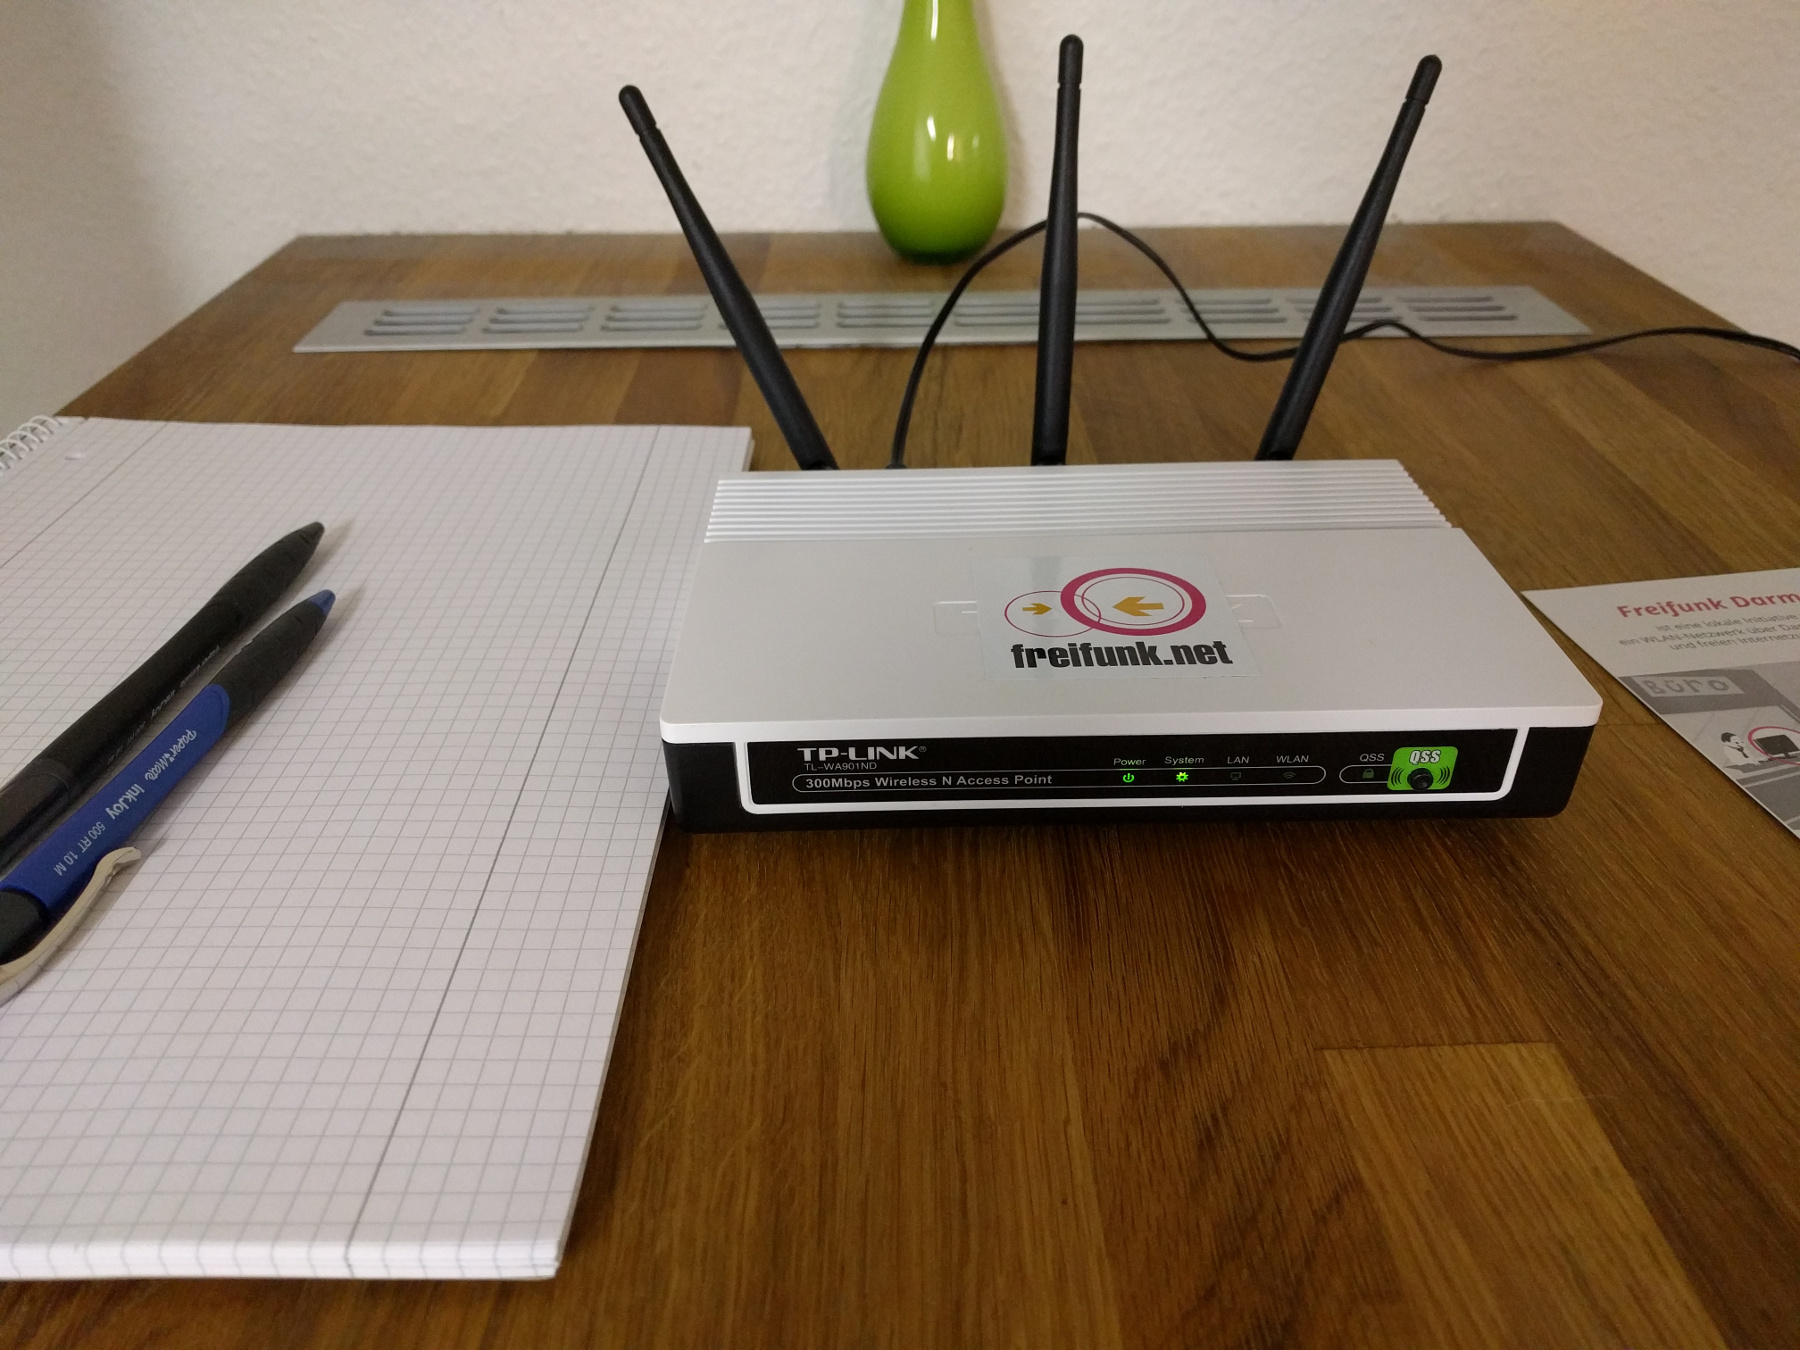
\includegraphics[width=7cm]{images/homerouter}
    \end{center}
  \end{frame}
  
  %-----------------
  \begin{frame}{Was ist Freifunk?}
    \begin{center}
      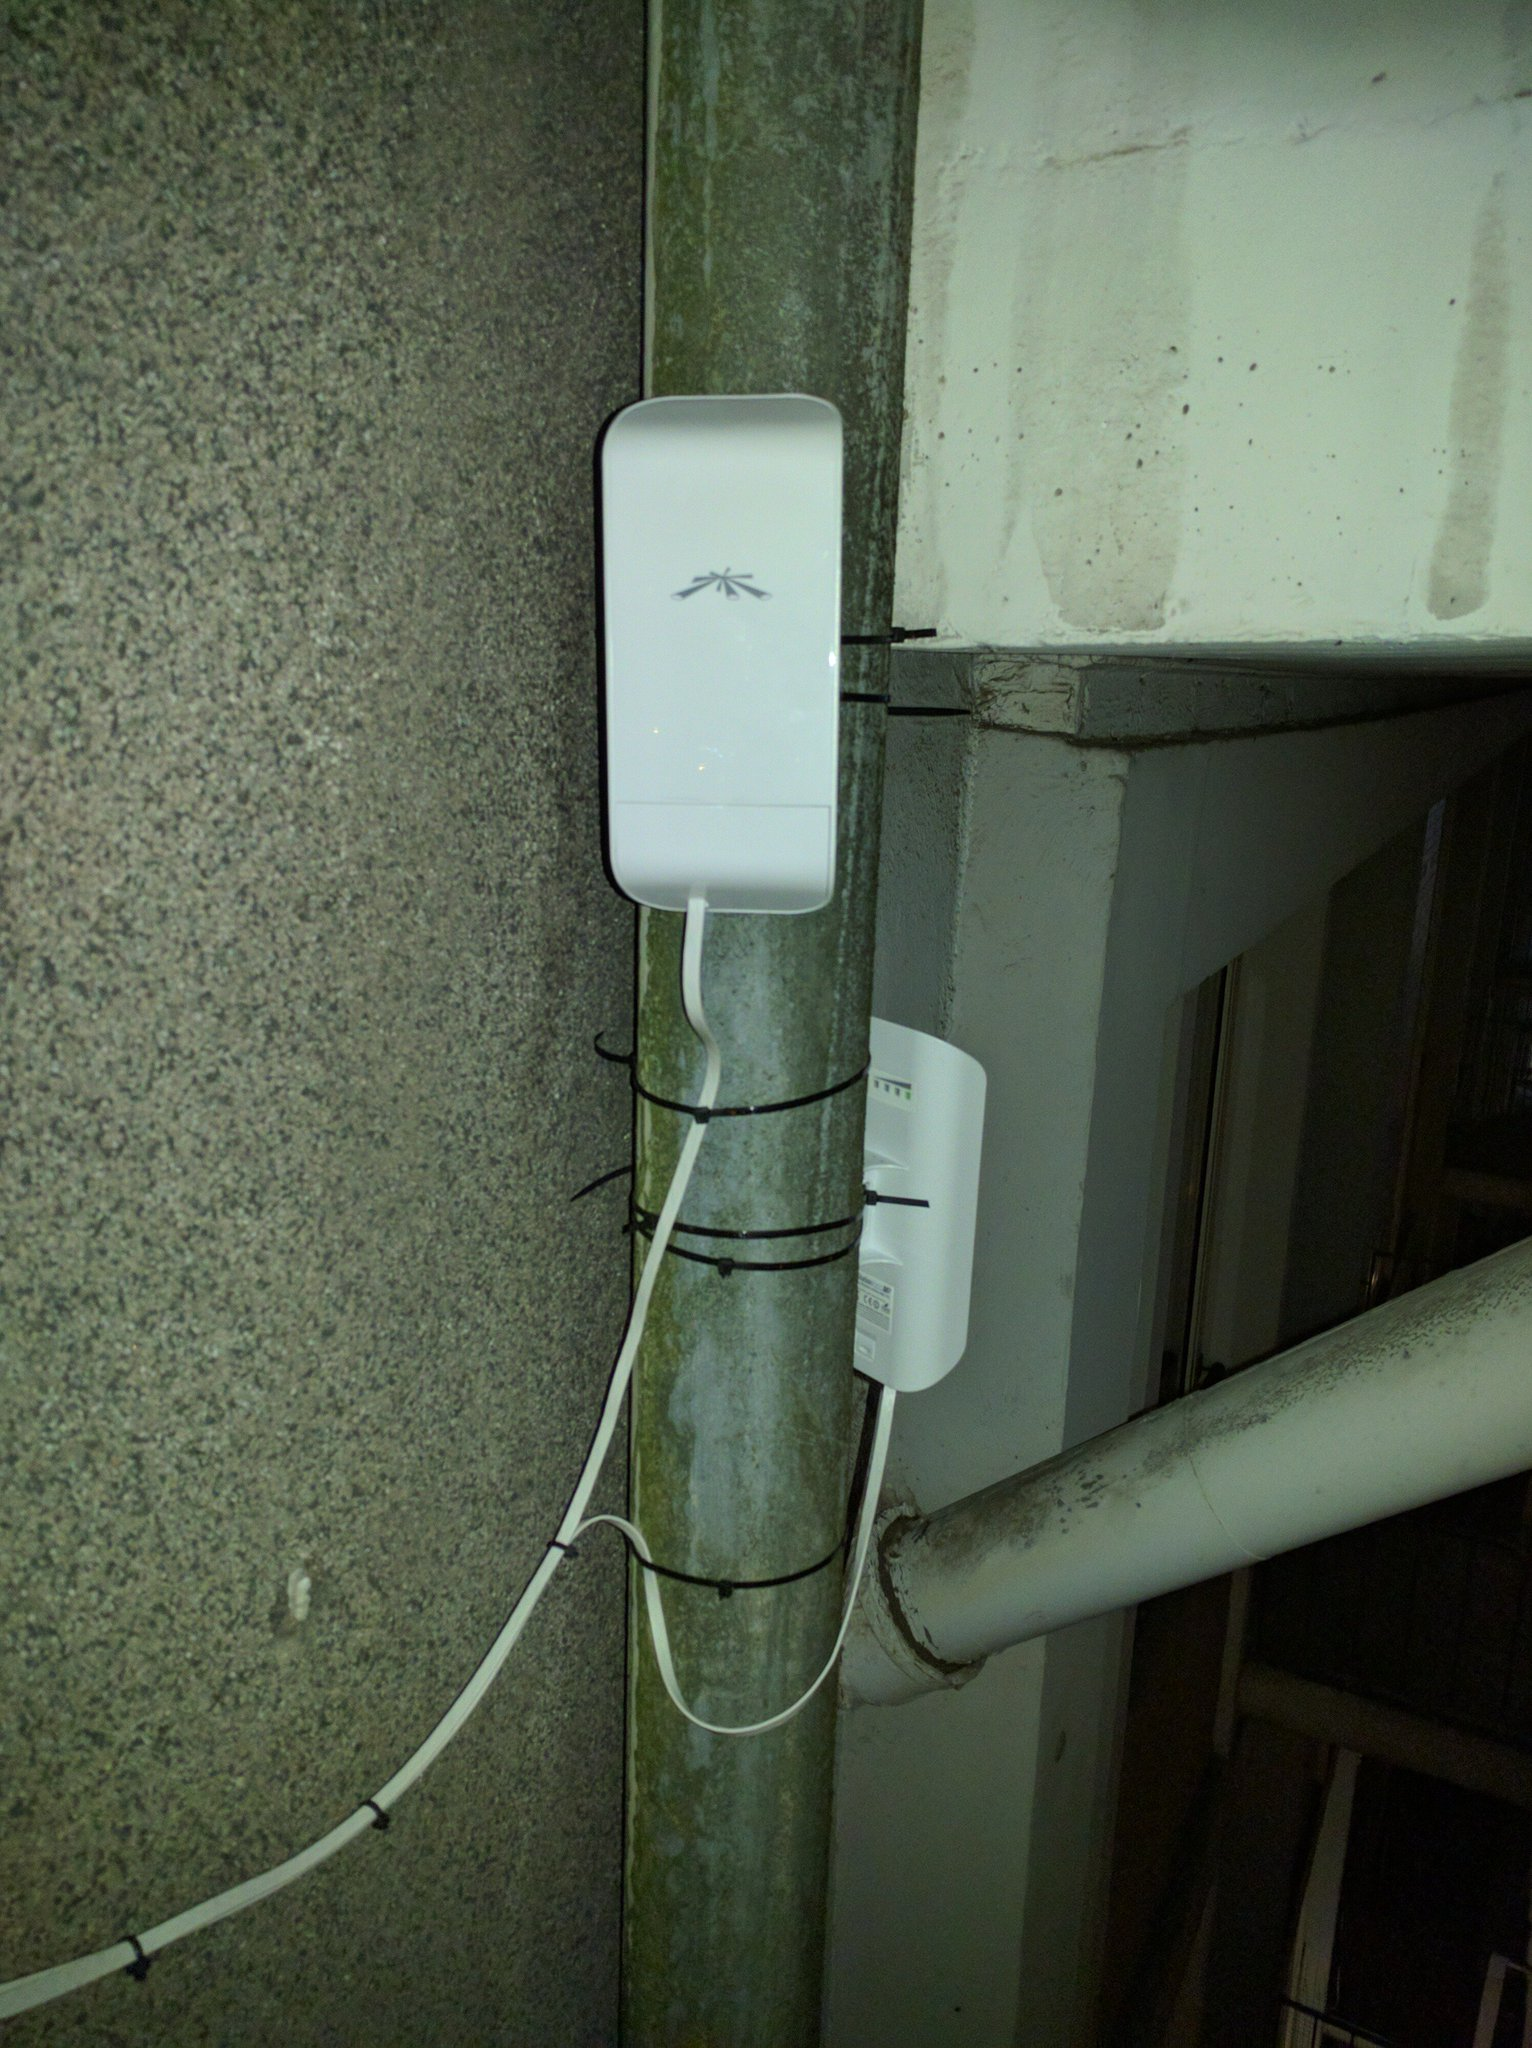
\includegraphics[width=5cm]{images/irl/wilhelminenstr2}
    \end{center}
  \end{frame}
  
  %-----------------
  \begin{frame}{Was ist Freifunk?}
    \begin{center}
      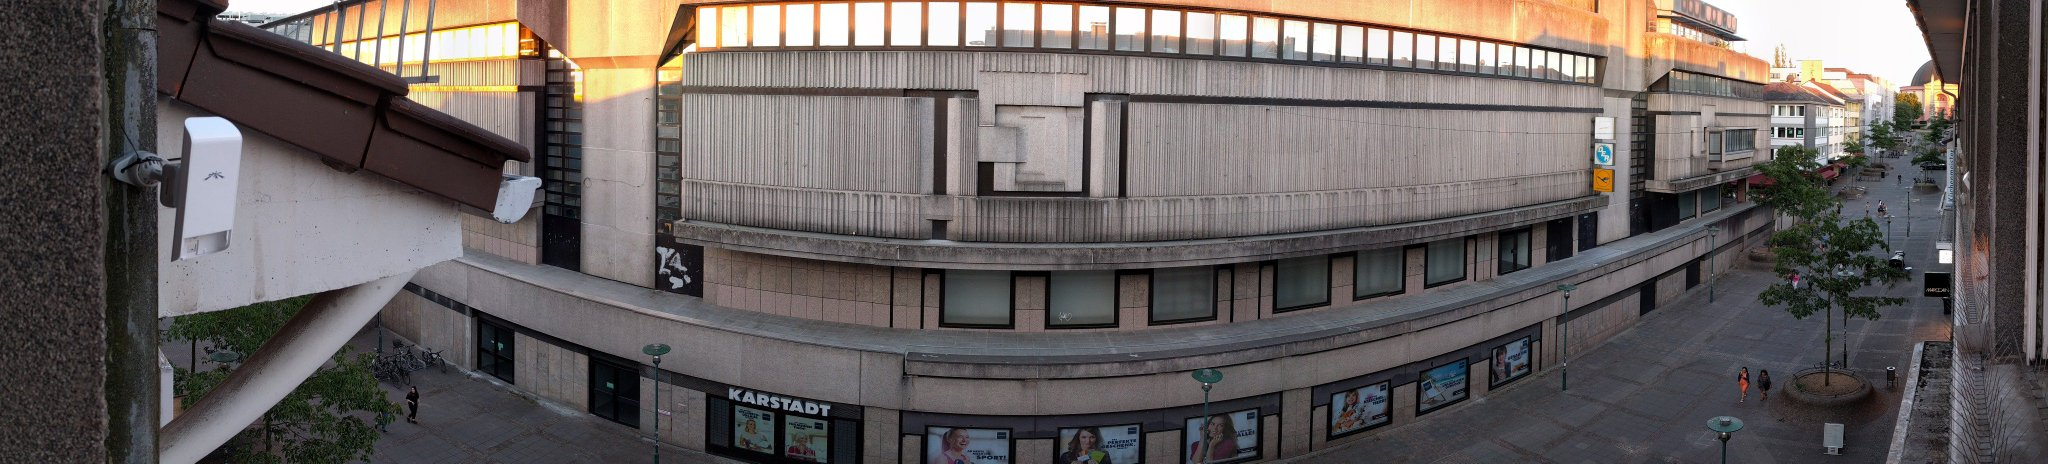
\includegraphics[width=10cm]{images/irl/wilhelminenstr1}
    \end{center}
  \end{frame}

  %-----------------
  \begin{frame}{Verbreitung}
    \begin{columns}
      \begin{column}{0.6\textwidth}
        \begin{itemize}
          \item Deutschlandweit über  \href{http://freifunk.net/wie-mache-ich-mit/community-finden/}{350 lokale Gruppen}
          \item mehr als 43.000 offene Zugangspunkte
        \end{itemize}
      \end{column}
      \begin{column}{0.4\textwidth}
        \begin{center}
          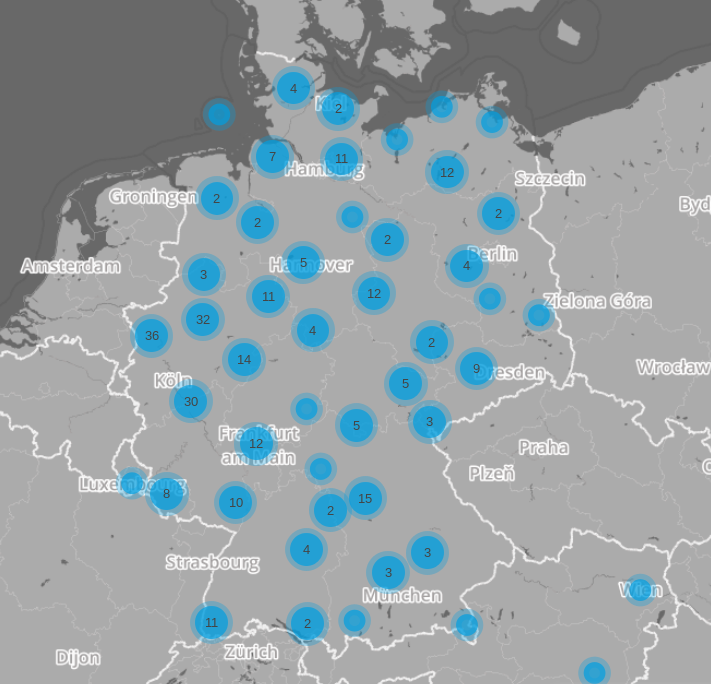
\includegraphics[width=\textwidth]{images/2016-06-01_map-de}
        \end{center}
      \end{column}
    \end{columns}
  \end{frame}

  %-----------------
  \begin{frame}{Ziele von Freifunk}
    \begin{itemize}
      \item \textbf{Beteiligung der Bevölkerung} an Aufbau und Entwicklung \textbf{dezentraler Netze}
      \item Verständnis von Kommunikationsnetzen fördern $\xRightarrow{}$ \textbf{Bildungsauftrag}
      \item Beteilung an gesellschaftlichen Initiativen, um die \textbf{Verbreitung freier Netze} zu unterstützen
    \end{itemize}
  \end{frame}


  %-----------------
  \begin{frame}{Stadt Darmstadt}
    \begin{itemize}
      \item Über 400 Freifunk-Router in Darmstadt
      \item Täglich über 1000 Nutzer gleichzeitig online
    \end{itemize}
  \end{frame}

  %-----------------
  \begin{frame}{Stadt Darmstadt}
    \begin{itemize}
      \item September 2015: Kooperation mit OB Partsch, Stadt Darmstadt vereinbart
      \item Bis Weihnachten wurden alle angefragten Unterkünfte mit WLAN versorgt
      \item Großartige Zusammenarbeit mit ASB, DRK, Feuerwehr und der städtischen IT
      \item IT Materialkosten < 5.000 \texteuro
    \end{itemize}
  \end{frame}

  %-----------------
  \begin{frame}{Stadt Babenhausen, Darmstadt-Dieburg}
    \begin{itemize}
      \item Versorgung eines Erstaufnahmelagers mit ca. 1.500 Personen in ehem. US-Kaserne
      \item Versorgung der Innenstadt entlang der Hauptachse über 1,8 km angestrebt
      \item Beratung des Bürgermeisters und tatkräftige Hilfe beim Aufbau einer Community
    \end{itemize}
  \end{frame}

  %-----------------
   \begin{frame}{Freifunk Darmstadt: In Zahlen}
    \begin{itemize}
	  \item ungefähr 1600 gleichzeitige Nutzer täglich
	  \item \emph{über} 600 Freifunk-Knoten in Darmstadt und Umland
	  \item über 155 TB an Internetverkehr \emph{jeden Monat}
    \end{itemize}
    \begin{center}
      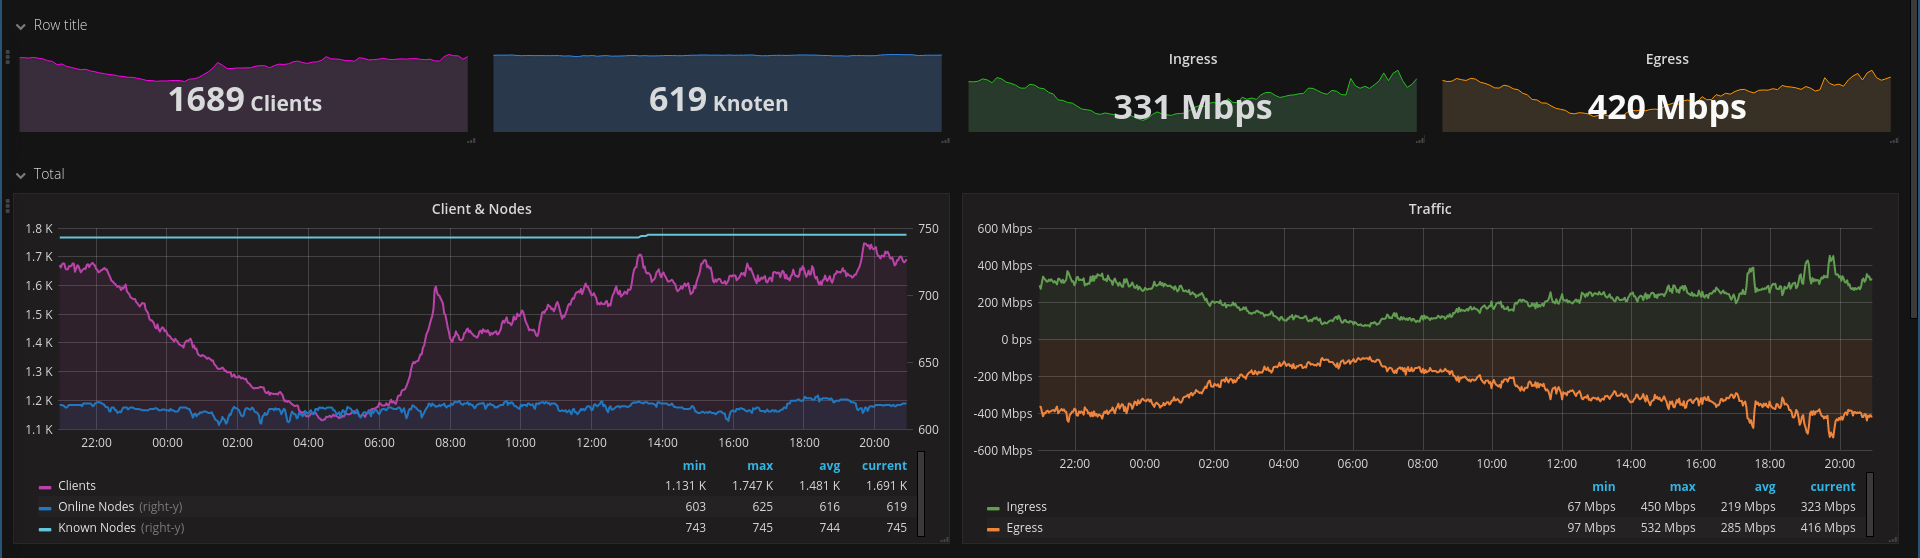
\includegraphics[height=3cm]{images/stats/grafana/2017_05_02}
    \end{center}
  \end{frame}

  %-----------------
  \begin{frame}{Störerhaftung}
    \begin{itemize}
      \item Keine Haftung für Knotenbetreiber
      \item Internetverkehr geht über unsere Gateways. Haftungsbefreiung nach TMG \S8.
      \item Wir nehmen die gesetzlichen Vorschriften wörtlich: Wir sammeln keine Daten.
    \end{itemize}
  \end{frame}

  %-----------------
  \begin{frame}{Richtfunknetz}
    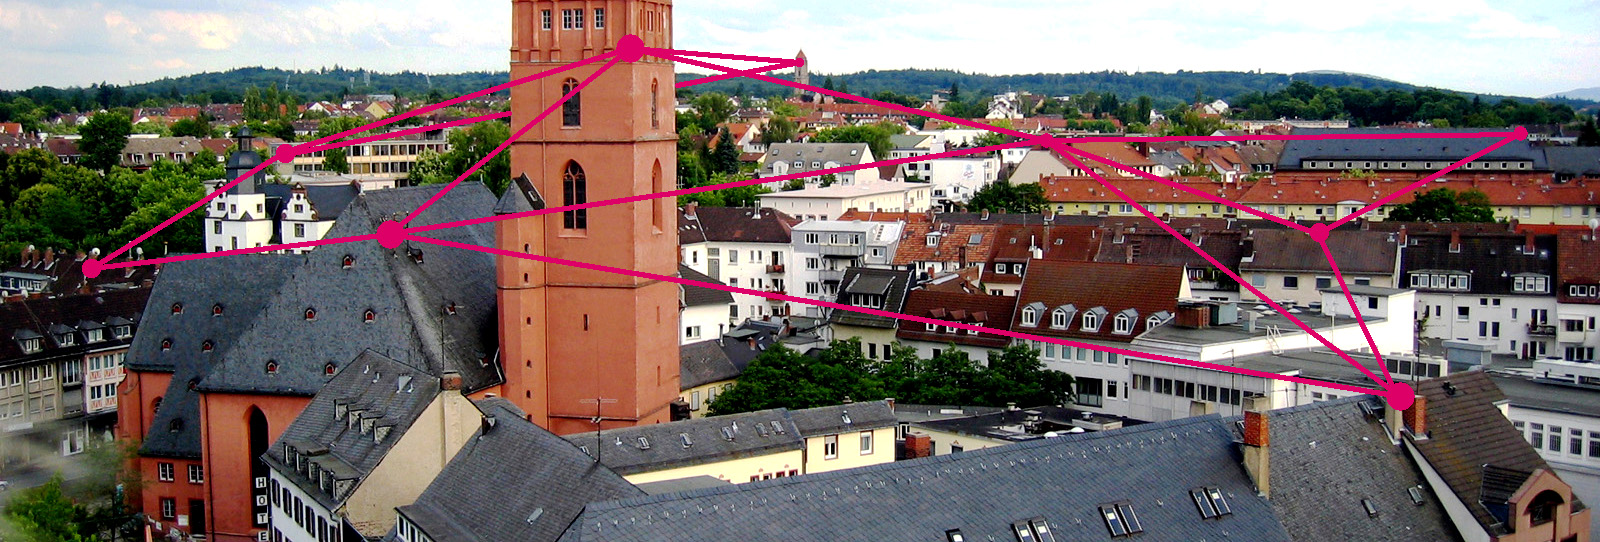
\includegraphics[width=\textwidth]{images/banner-stadtkirche-darmstadt}
    \begin{columns}
      \begin{column}{0.65\textwidth}
        \begin{itemize}
          \item Eigene Infrastruktur
          \begin{itemize}
            \item Redundanz und Lastverteilung
            \item Unabhängig vom Internet
          \end{itemize}
        \end{itemize}
      \end{column}
      \begin{column}{0.25\textwidth}
        \begin{center}
          \vspace{-1.5cm}
          \hspace{-0.75cm}
          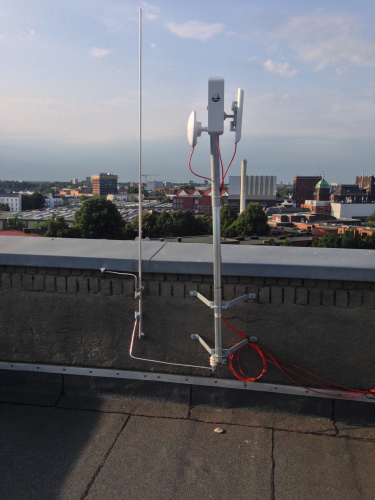
\includegraphics[width=\textwidth]{images/hamburg-richtfunkmast}
        \end{center}
      \end{column}
    \end{columns}
  \end{frame}

  %-----------------
  \begin{frame}{Kosten}
    \begin{itemize}
      \item Internetzugang durch Freifunker (\textbf{Privatpersonen}, Träger, Kommunen)
      \item Hardware je nach Nutzungsart ab 20,- €
      \item Kosten für Infrastruktur: Ca. 6,- \texteuro\ pro Router und Jahr
    \end{itemize}
  \end{frame}

  %-----------------

  \begin{frame}{Vielen Dank!}
    \begin{textblock*}{0cm}(\textwidth-2cm,-2cm)
      \begin{figure}[h]
        \def\svgwidth{2.5cm}
        \input{logo.pdf_tex}
      \end{figure}
    \end{textblock*}
      \begin{itemize}
        \item Webseite: \href{http://darmstadt.freifunk.net/}{darmstadt.freifunk.net}
        \item E-Mail: \href{info@darmstadt.freifunk.net}{info@darmstadt.freifunk.net}
        \item Treffen: Jeden Montag um 19:00 Uhr
      \end{itemize}
      \vspace{1em}
  \end{frame}
\end{document}
